\documentclass{beamer}
\mode<presentation> 
{
	\usetheme[alternativetitlepage]{Torino}
	\usecolortheme{chameleon}
	\setbeamercovered{transparent}	
}
\usepackage{ucs}
\usepackage[utf8x]{inputenc}
\usepackage[czech]{babel}
\usepackage{palatino}
\usepackage{graphicx}
\usepackage{epstopdf}
\usepackage{color}
\usepackage[export]{adjustbox}
\usepackage{multicol}
\usepackage{hyperref}
\usepackage{subcaption}
\usepackage{caption}
\captionsetup{labelformat=empty,labelsep=none}


\definecolor{olive}{RGB}{51, 149, 48}
\definecolor{red}{RGB}{195, 2, 36}

\definecolor{gred}{RGB}{196, 66, 48}
\definecolor{glime}{RGB}{168, 189, 4}
\definecolor{ggreen}{RGB}{57,181,74}

\title{\textbf{CUDA Raytracer}}
\author{
	\large{Pavel Macenauer} \\ 
	\tiny{xmacen02@stud.fit.vutbr.cz} \\ 
	\large{Jan Bureš} \\ 
	\tiny{xbures19@stud.fit.vutbr.cz}
}
\date{\tiny{\today}}
\institute[FIT VUTBR]
{
	\inst{}
	Fakulta Informačních Technologií \\
	Vysoké Učení Technické v Brně
}

\begin{document}

	\begin{frame}[t,plain]
	\titlepage
	\tableofcontents[currentsection]
	\vspace{-10mm}
	\center{ 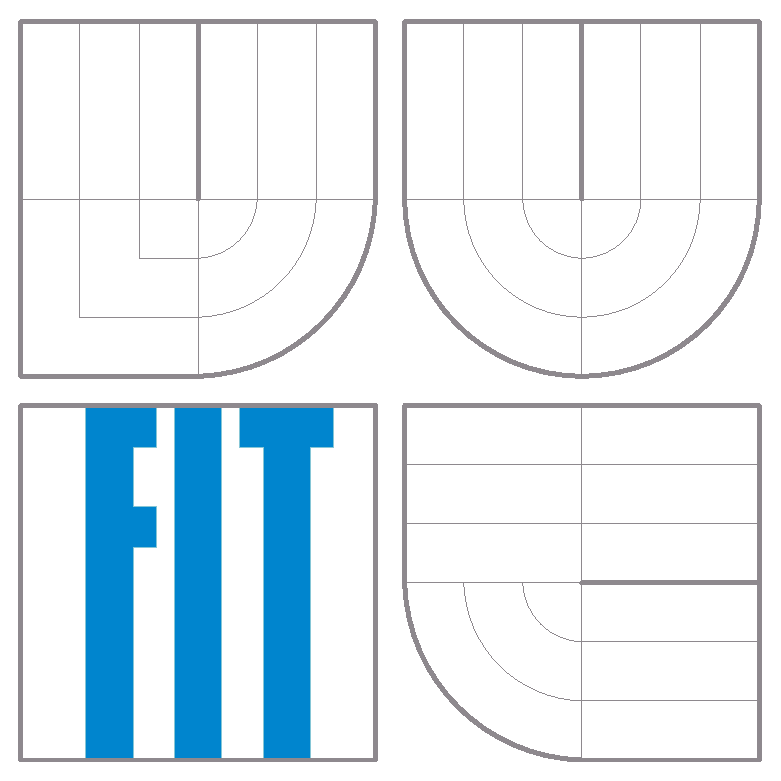
\includegraphics[height=9mm]{logo.eps} }
	\end{frame}

%% ------------- SNIMAC -------------

	\begin{frame}[t,fragile]
		\frametitle{Obsah}	
		
		\begin{itemize}
			\item Co náš raytracer umí?
			\item Použité technologie
			\item Rozvržení paměti
			\item Paralelizace
			\item Nápady na optimalizaci
			\item Srovnání s CPU			
		\end{itemize}			
				
	\end{frame}
	

	
	%% -----------------------------
	
	\begin{frame}[t,fragile]
		\frametitle{Co náš raytracer umí?}
		
		\begin{itemize}
			\item Jednoduchá primitiva \\
				\footnotesize{Koule, válec, rovina, trojúhelník}
			\item Phongův osvětlovací model
			\item Různé materiály (barva, lesk, \dots) včetně procedurální textury
			\item Načítání modelů ve formátu OBJ			
			\item Další vizuální vylepšení \\
			   \footnotesize{neostré stíny, hloubka ostrosti}			   
			\item akcelerace BVH, KD-tree
		\end{itemize}		
		
	\end{frame}


%% -----------------------------


	{
\usebackgroundtemplate{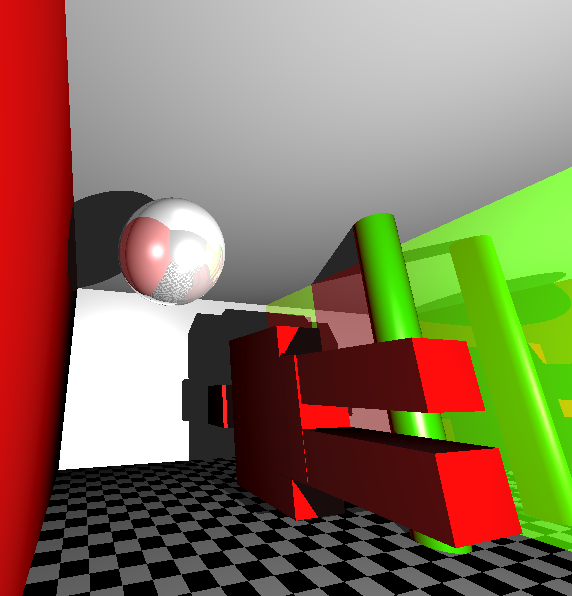
\includegraphics[width=\paperwidth]{img/complex.png}}
\begin{frame}[plain]
\end{frame}
}
	
%% ------------------------------

	\begin{frame}[t,fragile]
		\frametitle{Použité technologie}
		
		\begin{itemize}
			\item NVidia CUDA 6.5, \verb!C++11!
			\item Microsoft Visual Studio 2013 + NVidia NSight
			\item GLUT, GLEW
		\end{itemize}	
			

	\end{frame}
	
		%% --------------------------

	\begin{frame}[t,fragile]
		\frametitle{Rozvržení paměti}					
		\begin{itemize}
	\item světla (constant memory)
	\item nastavení kamery (constant memory)
	\item informace o~materiálech (constant memory)
	\item databáze primitiv (constant memory - \textit{???})
\end{itemize}
		
	
	\end{frame}
	
	%% --------------------------
	
		\begin{frame}[t,fragile]
		\frametitle{Paralelizace}	
				\vspace{15mm}				

\large
Pro každý pixel syntetizovaného obrazu se vyšle paprsek -- vytvoří vlákno a~to vypočte výslednou barvu (včetně odrazů a~stínů).


								
	\end{frame}	
	
	%% --------------------------
	
	\begin{frame}[t,fragile]
		\frametitle{Nápady na optimalizaci}
		\vspace{15mm}
		\begin{itemize}
	    	\item Odraz paprsku - nečekat až skončí, ale po každé rekurzi alokovat znovu vlákna
			\item Akcelerační struktury přímo na GPU
		\end{itemize}					
		
	\end{frame}
	
%% --------------------------

	\begin{frame}[t,fragile]
		\frametitle{Testovací scéna}					
		
		\begin{itemize}
	\item počet rovin: \textbf{6}
	\item počet koulí: \textbf{5, 10, 20, 50, 100, 500}
	\item hardware: \textbf{NVidia Quadro K1000M, Intel Core i7-3610QM 2.3 GHz}
\end{itemize}

	\begin{figure}[htbp]
        \centering

        \begin{subfigure}[b]{0.49\textwidth}
                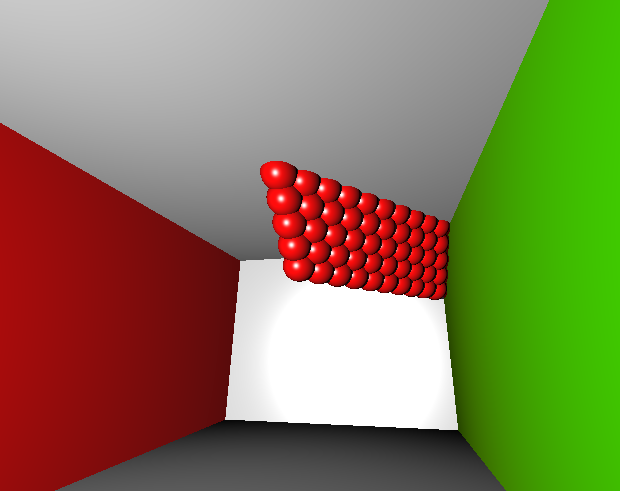
\includegraphics[width=\textwidth]{img/test-scene.png}
                \caption{\scriptsize{CUDA}}
        \end{subfigure}   
        \begin{subfigure}[b]{0.49\textwidth}
                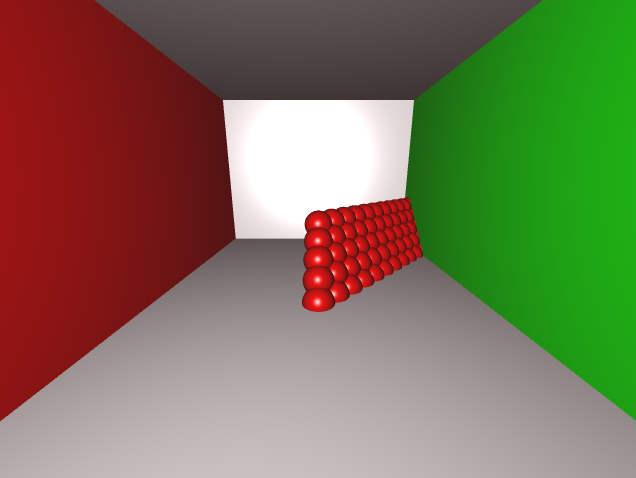
\includegraphics[width=\textwidth]{img/test-scene-aurelius.png}
                \caption{\scriptsize{Aurelius}}

        \end{subfigure}
        
        \end{figure}

	\end{frame}
	
	

	
		%% --------------------------
	
		\begin{frame}[t,fragile]
		\frametitle{Výsledky}					
		\small
		\begin{table}
\centering
\begin{tabular}{ | l | l | l | l | l | l | l |}
\hline
\textbf{Počet koulí} & 5  & 10  & 20 & 50 & 100 & 500 \\
\hline
\textbf{CUDA} [s] & 0,0193 & 0,0195 & 0,0224 & 0,0341 & 0,05521 & 0,2197 \\
\hline
\textbf{Aurelius} [s] & 0,905 & 1,233 & 1,779 & 3,541 & 6,505 & 30,373 \\
\hline
\end{tabular}
\caption{Srovnání podobně komplexních scén na raytraceru Aurelius a~CUDA raytraceru pro daný počet koulí}
\end{table}

Syntéza raytracerem Aurelius byla cca 100x pomalejší, než-li syntéza podobné scény na GPU. S~komplexností scény se rozdíly mezi CPU a GPU verzí ještě zvětšují.

	\end{frame}
	
		%% --------------------------
		
				{
\usebackgroundtemplate{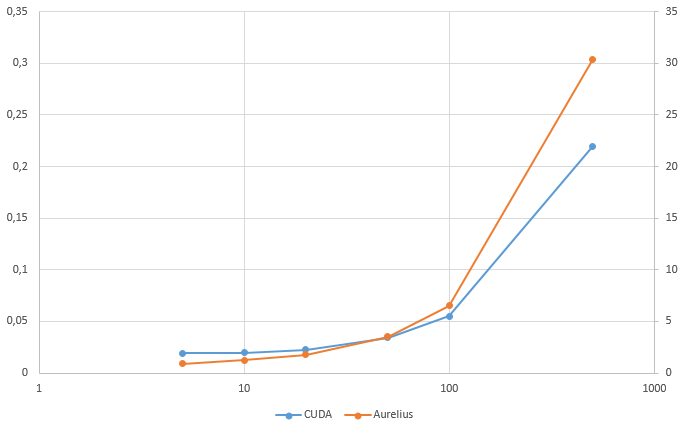
\includegraphics[width=\paperwidth]{img/srovnani.png}}
\begin{frame}[plain]
\end{frame}
}

	\begin{frame}[t,fragile]

		\vspace{30mm}
\centering
\Huge Děkujeme za pozornost.\\ Otázky?
						
		
	\end{frame}

	
\end{document} 
